%%%%%%%%%%%%%%%%%%%%%%%%%%EJERCICIO 12 %%%%%%%%%%%%%%%%%%%%%%%%%%%
\textbf{Ejemplo 12}\\
Se desean reunir 800{.}000 \; \text{COP} en 4 depósitos periódicos trimestre vencido crecientes en un 20\% más una cuota extra pactada de 80{.}000 \; \text{COP} en el período 2 trimestre vencido. Con una tasa del 20\% período trimestre vencido. Elabore la tabla de capitalización.\\

\textbf{Solución 12}\\
% La tabla irá centrada
\begin{center}
	\renewcommand{\arraystretch}{1.5}% Márgenes de las celdas
	% Creación de la cuadrícula de 3 columnas
	\begin{longtable}[H]{|c|c|c|}
		% Creamos una línea horizontal
		\hline
		% Definimos el color de la primera fila
		\rowcolor[HTML]{FFB183}
		\hline
		%%%%% INICIO ASIGNACIÓN PERÍODO FOCAL %%%%%%%
		%%%%%%%%%% INICIO TÍTULO
		% Lo que se hace aquí es mezclar las 3 columnas en una sola
		\multicolumn{3}{|c|}{\cellcolor[HTML]{FFB183}\textbf{1. Asignación período focal}} \\ \hline
		%%%%%%%%%% FIN TÍTULO
		%%%%% INICIO DECLARACIÓN DE VARIABLES %%%%%%%
		\multicolumn{3}{|c|}{$pf : 5 \; \textit{ptv}$} \\ \hline
		%%%%%%%%%% INICIO TÍTULO
		% Lo que se hace aquí es mezclar las 3 columnas en una sola
		\multicolumn{3}{|c|}{\cellcolor[HTML]{FFB183}\textbf{2. Declaración de variables}} \\ \hline
		\hline
		%%%%%%%%%% FIN TÍTULO
		%%%%%%%%%% INICIO DE MATEMÁTICAS
		\cellcolor[HTML]{FFB183}\textbf{Valores monetarios} & 
		\cellcolor[HTML]{FFB183}\textbf{Valores no monetarios} & 
		\cellcolor[HTML]{FFB183}\textbf{Incógnitas} \\ \hline
		$VF = 800{.}000 \; \text{COP}$ & $g = 20\%$ & $R_{1} = ? \; \text{COP}$ \\ 
		$R = 80{.}000 \; \text{COP}$ & $n = 4 \; \textit{ptv}$ & \\ 
		$ $ & $i = 20\% \; \textit{ptv}$ & \\ \hline
		%%%%%%%%%% FIN DE MATEMÁTICAS
		%%%%% FIN DECLARACIÓN DE VARIABLES

		\rowcolor[HTML]{FFB183}
		\hline
		\multicolumn{3}{|c|}{\cellcolor[HTML]{FFB183}\textbf{3. Diagrama de flujo de caja}} \\ \hline
		\multicolumn{3}{|c|}{ 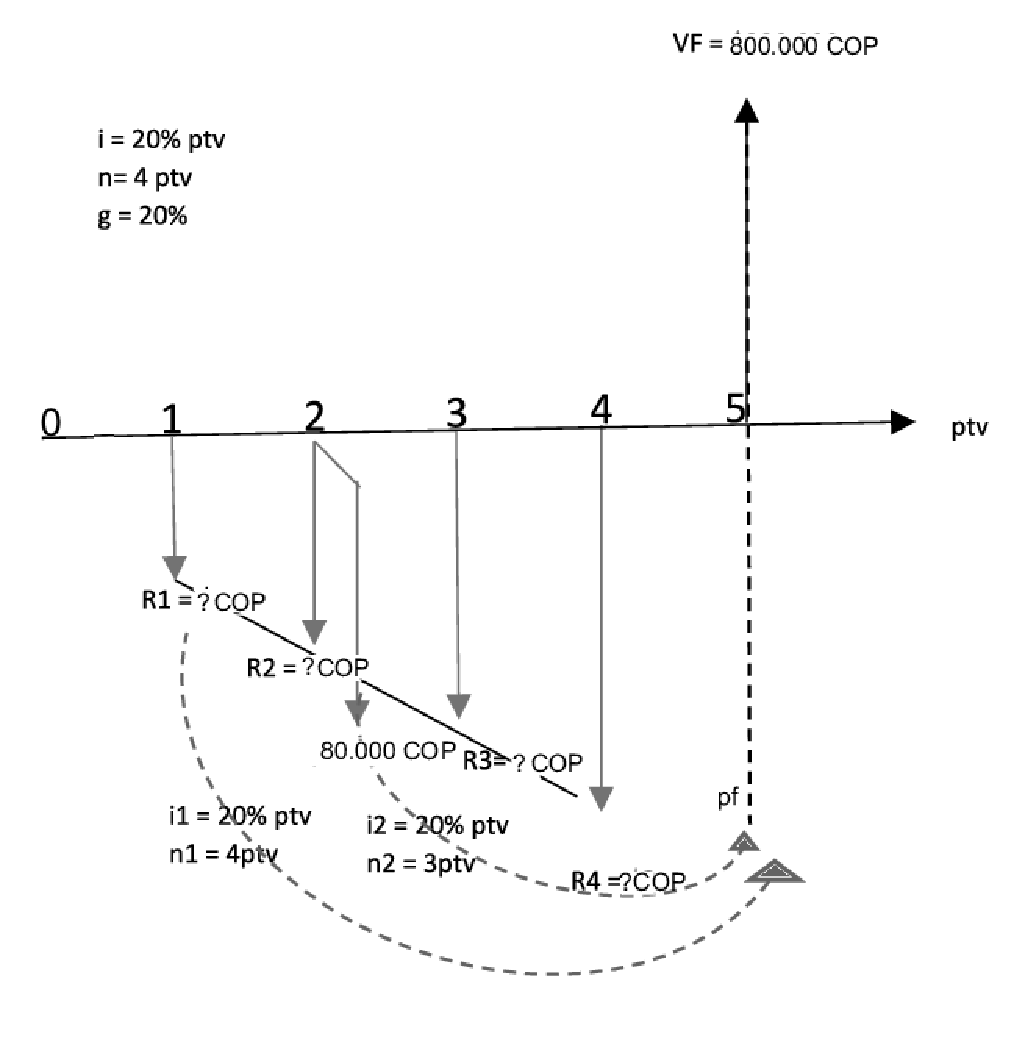
\includegraphics[trim=-78 -5 -78 -5, width=14cm]{7_Capitulo/img/ejemplos/12/12_1.pdf} } \\ \hline
		%%%%% INICIO FLUJO DE CAJA
		\rowcolor[HTML]{FFB183}
		\hline
		\multicolumn{3}{|c|}{\cellcolor[HTML]{FFB183}\textbf{4. Declaración de fórmulas}} \\ \hline
		%%%%%%%%%%%%% FIN INSERCIÓN DE IMAGEN
		%%%%% FIN FLUJO DE CAJA

		\multicolumn{3}{|c|}{ $VF = R_{1} n (1+i)^{n-1} + R (1+i)^{2}$ Valor futuro de un Gradiente Geométrico } \\ \hline
		
		%%%%%% INICIO DESARROLLO MATEMÁTICO
		\rowcolor[HTML]{FFB183}
		\hline
		%%%%%%%%%% INICIO TÍTULO
		\multicolumn{3}{|c|}{\cellcolor[HTML]{FFB183}\textbf{5. Desarrollo matemático}} \\ \hline
		%%%%%%%%%% FIN TÍTULO
		%%%%%%%%%% INICIO MATEMÁTICAS
		\multicolumn{3}{|c|}{ $800{.}000 \; \text{COP} = R_{1} \cdot 4 \cdot (1 + 0{.}2)^{3} + 80{.}000 \; \text{COP} \cdot (1 + 0{.}2)^{2}$ } \\ 
		\multicolumn{3}{|c|}{ $R_{1} = 99{.}074{,}07 \; \text{COP}$ } \\ 
		\multicolumn{3}{|c|}{ $R_{2} = 99{.}074{,}07 \; \text{COP} \cdot (1 + 0{.}2)^{1} + 80{.}000 \; \text{COP} = 198{.}888{,}89 \; \text{COP}$ } \\ 
		\multicolumn{3}{|c|}{ $R_{3} = 99{.}074{,}07 \; \text{COP} \cdot (1 + 0{.}2)^{2} = 142{.}666{,}67 \; \text{COP}$ } \\ 
		\multicolumn{3}{|c|}{ $R_{4} = 99{.}074{,}07 \; \text{COP} \cdot (1 + 0{.}2)^{3} = 171{.}200{,}00 \; \text{COP}$ } \\ \hline

		%%%%%%%%%% FIN MATEMÁTICAS
		%%%%%% FIN DESARROLLO MATEMÁTICO
		%%%%%% INICIO RESPUESTA
		\rowcolor[HTML]{FFB183}
		\hline
		%%%%%%%%%% INICIO TÍTULO
		\multicolumn{3}{|c|}{\cellcolor[HTML]{FFB183}\textbf{6. Respuesta}} \\ \hline
		%%%%%%%%%% FIN TÍTULO
		%%%%%%%%%% INICIO RESPUESTA MATEMÁTICA
		\multicolumn{3}{|c|}{ 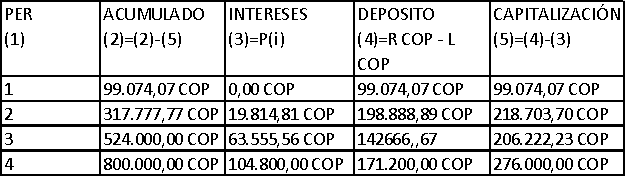
\includegraphics[trim=-78 -5 -78 -5]{7_Capitulo/img/ejemplos/12/12_2.pdf} } \\ \hline
	\end{longtable}
	% Se crean dos líneas en blanco para que no quede el siguiente texto tan pegado
	%\newline \newline % USARLO SI CREES QUE ES NECESARIO
\end{center}
%%%%%%%%%%%%%%%%%%%%%%%%%%FIN EJERCICIO 12 %%%%%%%%%%%%%%%%%%%%%%%%%%%
